\documentclass[12pt,a4paper]{article}
\usepackage{amsmath,amscd,amsbsy,amssymb,latexsym,url,bm,amsthm}
\usepackage{epsfig,graphicx,subfigure}
\usepackage{enumitem,balance}
\usepackage{wrapfig}
\usepackage{mathrsfs,euscript}
\usepackage[usenames]{xcolor}
\usepackage{hyperref}
\usepackage{float}
\usepackage[vlined,ruled,linesnumbered]{algorithm2e}
\hypersetup{colorlinks=true,linkcolor=black}

\newtheorem{theorem}{Theorem}
\newtheorem{lemma}[theorem]{Lemma}
\newtheorem{proposition}[theorem]{Proposition}
\newtheorem{corollary}[theorem]{Corollary}
\newtheorem{exercise}{Exercise}
\newtheorem*{solution}{Solution}
\newtheorem{definition}{Definition}
\theoremstyle{definition}

\renewcommand{\thefootnote}{\fnsymbol{footnote}}

\newcommand{\postscript}[2]
 {\setlength{\epsfxsize}{#2\hsize}
  \centerline{\epsfbox{#1}}}

\renewcommand{\baselinestretch}{1.0}

\setlength{\oddsidemargin}{-0.365in}
\setlength{\evensidemargin}{-0.365in}
\setlength{\topmargin}{-0.3in}
\setlength{\headheight}{0in}
\setlength{\headsep}{0in}
\setlength{\textheight}{10.1in}
\setlength{\textwidth}{7in}
\makeatletter \renewenvironment{proof}[1][Proof] {\par\pushQED{\qed}\normalfont\topsep6\p@\@plus6\p@\relax\trivlist\item[\hskip\labelsep\bfseries#1\@addpunct{.}]\ignorespaces}{\popQED\endtrivlist\@endpefalse} \makeatother
\makeatletter
\renewenvironment{solution}[1][Solution] {\par\pushQED{\qed}\normalfont\topsep6\p@\@plus6\p@\relax\trivlist\item[\hskip\labelsep\bfseries#1\@addpunct{.}]\ignorespaces}{\popQED\endtrivlist\@endpefalse} \makeatother

\begin{document}
\noindent

%========================================================================
\noindent\framebox[\linewidth]{\shortstack[c]{
\Large{\textbf{Lab03-Greedy Strategy}}\vspace{1mm}\\
CS214-Algorithm and Complexity, Xiaofeng Gao, Spring 2021.}}


\begin{center}
\footnotesize{\color{red}$*$ If there is any problem, please contact TA Haolin Zhou.}\par
% Please write down your name, student id and email.
\footnotesize{\color{blue}$*$ Name:BeichenYu  \quad Student ID:519030910245 \quad Email:polarisybc@sjtu.edu.cn}
\end{center}

\begin{enumerate}
	\item \textit{Interval Scheduling.} Interval Scheduling is a classic problem solved by \textbf{greedy algorithm}: given $n$ jobs and the $j$-th job starts at $s_j$ and finishes at $f_j$. Two jobs are compatible if they do not overlap. The goal is to find maximum subset of mutually compatible jobs. Tim wants to solve it by sort the jobs in descending order of $s_j$. Is this attempt correct? Prove the correctness of such idea, or else provide a counter-example.
	    \begin{solution}
	        This idea is correct. In the common greedy strategy, we sort the jobs in ascending order of $f_j$. In fact, the idea of Tim is as same as the common strategy. In this problem we don't care the direction of time, and the only thing we care is the collision. If we let time go upstream, the two strategies will transform each other.\\
	        
	        Assume the idea of Tim is not optimal.
	        
	        Let $i_1,i_2,\cdots,i_k$ denote set of jobs selected by the idea of Tim.
	        
	        Let $j_1,j_2,\cdots,j_k$ denote set of jobs in an optimal solution with $i_k=j_k,i_{k-1}=j_{k-1},\cdots,i_{r}=j_r$ for the smallest possible value of $r$.
	        
	        So $i_{r-1}$ starts later than $j_{r-1}$. However, if we replace $j_{r-1}$ with $i_{r-1}$, solution is still feasible and optimal because interval scheduled before in the optimal solution can also be scheduled although the exchange happened. And that contradicts the minimality of r. 
	        
	        So the assumption doesn't hold, and the idea of Tim is optimal.
	    \end{solution}
	
	\item \textit{Done deal.} In a basketball league, teams need to complete player trades through matching contracts. Every player is offered a contract. For the sake of simplicity, we assume that the unit is $ M $, and the size of all contracts are integers. The process of contract matching refers to the equation: $ \sum_{i\in A} a_{i}=\sum_{j\in B} b_{j} $, where $ a_{i} $ refers to the contract value of player $ i $ in team $A$ involved in the trade and $ b_{j} $ refers to the value of player $ j $ in team $B$. 
	
	Assume that you are a manager of a basketball team and you want to get \textbf{one} star player from another team through trade. The contract of the star player is $ n (n\in \mathbb{N}^+) $. The goal is to complete the trade with as few players as possible. 
	
	\begin{enumerate}
		\item Describe a \textbf{greedy} algorithm to get the deal done with the least players in your team. Assume that there are only 4 types of contracts in your team: $25M$, $ 10M $, $ 5M $, $ 1M $, and there is no limit to the number of players. Prove that your algorithm yields an optimal solution.
		\item Suppose that the available contract sizes are powers of $c$,
		i.e., the values are $c^{0}, c^{1}, \ldots, c^{k}$ for some integers $c>1$ and $k \geq 1$. Show that the greedy algorithm always yields an optimal solution.
		\item Give a set of contract sizes for which the greedy algorithm does not yield an optimal solution. Your set should include a $ 1M $ so that there is a solution for every value of $ n $.
	\end{enumerate}
    \begin{solution}
        \begin{enumerate}
        \item First choose as many $25M$ contacts as possible. When the remain contacts is less then $25M$, choose as many $10M$ contacts as possible. When the remain contacts is less then $10M$, choose as many $5M$ contacts as possible. When the remain contacts is less then $5M$, use enough $1M$ contracts to fill up.
        
        First let us assume that if using this greedy algorithm, $n = m_1\times 1M+m_2\times 5M+m_3\times 10M+ m_4 \times 25M$. $m_1 < 5$ is obvious because if we have 5 players with a $1M$ contact, a player with a $5M$ contract is a better choice. For the same result, $m_2 < 2$, and 2 of $10M$ player can not exist together with a $5M$ player. We proof that the number of $25M$ must be $m_3$. We assume that there is a better algorithm and $n = p_1\times 1M+p_2\times 5M+p_3\times 10M+ p_4 \times 25M$. Because we use the greedy algorithm, $m_3 \geqslant p_3$. But if $p_3<m_3$, there is at least $25M$ must use $1M,5M$ and $10M$ to get. But it is impossible because we have at most 4 of $1M$ players, 1 of $5M$ player and available $10M$ players. So $m_3 = p_3$. Using the same method, we can proof that $m_2 = p_2, m_1 = p_1$ and $m_0 = p_0$. That is to say that the greedy algorithm is right. 
        
        \item If using the greedy algorithm, $n = m_0c^0 + m_1c^1 + \cdots + m_kc^k$ and we assume that there is a better algorithm, $n = n_0c^0 + n_1c^1 + \cdots + n_kc^k$. 

First, we proof that $n_k = m_k$. As it is a greedy algorithm, $m_k \geqslant n_k$. If $n_k < m_k$, then $n_k \leqslant m_k – 1$.
It is absolutely that $n_0, n_1, \cdots, n_{k-1} < c$ as if there is $c$ contracts they can be changed to a bigger contract. So $n_0c^0 + n_1c^1 + \cdots + n_{k-1}c^{k-1} \leqslant (c - 1)c^0 + (c - 1)c^1 + … + (c - 1)c^{k-1} = c^k – 1 < c^k$. So $n = n_0c^0 + n_1c^1 + \cdots + n_kc^k < c^k + n_kc^k <= m_kc^k < n$, and it is absolutely wrong. So $n_k = m_k$.

Using the same method, we can proof that for $\forall i \leqslant k, n_i = m_i$. That is to say that the greedy algorithm is correct.

\item Assume that there are only 3 types of contracts in your team: $ 8M $, $ 5M $, $ 1M $, and $n = 20M$. If using the greedy algorithm, the solution should be $8 \time 8M + 4\times 1M$, 6 players in total. This is not the optimal obviously as $4\times 5M$ can solve it as well. 

        \end{enumerate}
    \end{solution}
	
    \item \textit{Set Cover.} \textbf{Set Cover} is a typical kind of problems that can be solved by greedy strategy. One version is that: Given $n$ points on a straight line, denoted as $\{x_i\}_{i=1}^n$, and we intend to use minimum number of closed intervals with fixed length $k$ to cover these $n$ points.
    \begin{enumerate}
    	\item Please design an algorithm based on \textbf{greedy} strategy to solve the above problem, in the form of \emph{pseudo code}. Then please analyze its \emph{worst-case} complexity.
    	\item Please prove the correctness of your algorithm.
    	\item Please complete the provided source code by C/C++, and please write down the output result by testing the following inputs: 
    	\begin{enumerate}
    		\item the number of points $n=7$;
    		\item the coordinates of points
    		$x=\{1,2,3,4,5,6,-2\}$;
    		\item the length of intervals
    		$k=3$.
    	\end{enumerate}
        \textbf{Remark}: Screenshots of running results are also acceptable 
    \end{enumerate}
    \begin{solution}
        \begin{enumerate}
        \item The pseudo code is as follows.\\
        \begin{minipage}[t]{0.88\textwidth}
        \begin{algorithm}[H]
		\caption{Set Cover}\label{Alg-SetCover}
		
		Sort the coordinates of points so that $x_1\leqslant x_2\leqslant \cdots \leqslant x_n$;
		
		$ans \leftarrow 1$; $index \leftarrow 1$; $left \leftarrow x_1$; $right \leftarrow left+k$\;
		\While{$index < n$}{
		    $index \leftarrow index+1$\;
			\If{$x[index] > right$}{
				$ans \leftarrow ans+1$\;
				$left \leftarrow x[index]$;
				$right \leftarrow left + k$;
			}
		}
		return $ans$;
	\end{algorithm}
	
	In the sorting part, the time complexity in the worst case is $O(n^2)$. And when doing the loop the time complexity is always $O(n)$, so finally the time complexity in the worst case is $O(n^2)$.
	\end{minipage}
	
	\item Assume the idea of Tim is not optimal.
	        
	      Let $l_1,l_2,\cdots,l_k$ denote intervals selected by the greedy algorithm. 
	      
	      Let $s_1,s_2,\cdots,s_k$ denote intervals selected by an optimal solution with $l_1=s_1,l_{2}=s_{2},\cdots,l_{r}=s_r$ for the biggest possible value of $r$.
	      
	      So the left endpoint of $s_{r+1}$ is smaller then $l_{r+1}$. However, if we replace $s_{r+1}$ with $i_{r+1}$, solution is still feasible and optimal because the points after the interval can still be covered although the exchange happened. And that contradicts the maximality of r. 
	      
	      So the assumption doesn't hold, and the greedy algorithm is optimal.
	      
	\item I have finish it and the source code is included in the zip. The output is 3, and the screenshot of running results is below.
	
	\begin{figure}[H]
    \centering
    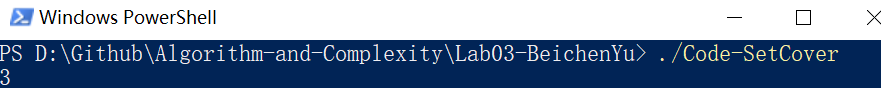
\includegraphics[width=0.8\textwidth]{result.png}
    \caption{The screenshot of running results}
\end{figure}
	
	
        \end{enumerate}
    \end{solution}

\end{enumerate}



\vspace{20pt}

\textbf{Remark:} You need to include your .pdf and .tex files in your uploaded .rar or .zip file.

%========================================================================
\end{document}
